\chapter{Návrh riešenia problému}
\section{Existujúce problémy}
Pred zahájením tvorby aplikácie je nutné oboznámiť sa s problémami, ktoré je nutné aby aplikácia riešila. Na prvý pohľad  sa môže zdať, že  počítanie ľudí je jednoduchý proces. Predpokladajme, že virtuálna brána je umiestnená pri vstupe do miestnosti. Proces prechodu osoby znamená zvýšenie počítadla prechodov osôb a na základe smeru danej osoby dekrementovať alebo inkrementovať počet osob nachádzajúcich sa v miestnosti. Systém musí byť navrhnutý tak, aby bol schopný detekovať a sledovať aj viacero ľudí ktorý v jedenom okamihu prechádzajú cez virtuálnu bránu rovnakým alebo odlišným smerom.  Jeden z najväčších problémov je však dynamickosť prostredia, kde by aplikácia mala byť nasadená. Rýchle svetelné zmeny okolia,  nepredvídateľné pohyby ľudí na scéne (môže zastať, dotýkať sa, ťahať / tlačiť iný objekt)  toto všetko je nutné riešiť, tak aby aplikácia dosiahla čo najväčšej presnosti. 

\section{Konceptuálny návrh systému}
Z problémov opísaných v sekcii 3.1 je jasné, že jednoduché systémy typu Infračervená závora, nebudú mať dostatočne veľkú presnosť vzhľadom na prechody viacerých osôb v jednom časovom okamihu. Je nutné oprieť sa o metódy, ktoré vedia zaznamenať viac informácii o objekte, ktorý prechádza vymedzeným priestorom (tvar, rýchlosť, veľkosť, smer, atd …). 

Jedným z najkomplexnejších prostriedkov, ako dostať dáta do počítača na spracovanie je kamera, ktorá nám poslúži ako senzor.  Umiestnime ju na vrchnú priečku prechodu tak, aby snímala osoby z vrchu. Táto pozícia je najlepšia, lebo eliminuje možnosti zatienenia sledovaného objektu iným objektom na scéne.  

\begin{figure}[H]
  \centering
  \begin{minipage}[b]{0.2\textwidth}
    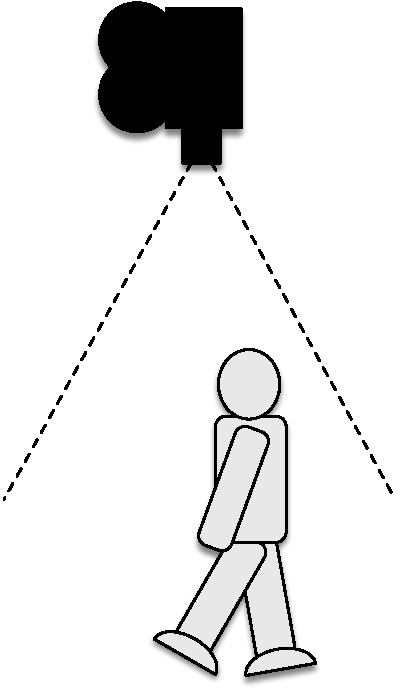
\includegraphics[width=\textwidth]{images/conceptCameraPos}
    \caption{Poloha kamery.}
  \end{minipage}
  \hfill
  \begin{minipage}[b]{0.5\textwidth}
    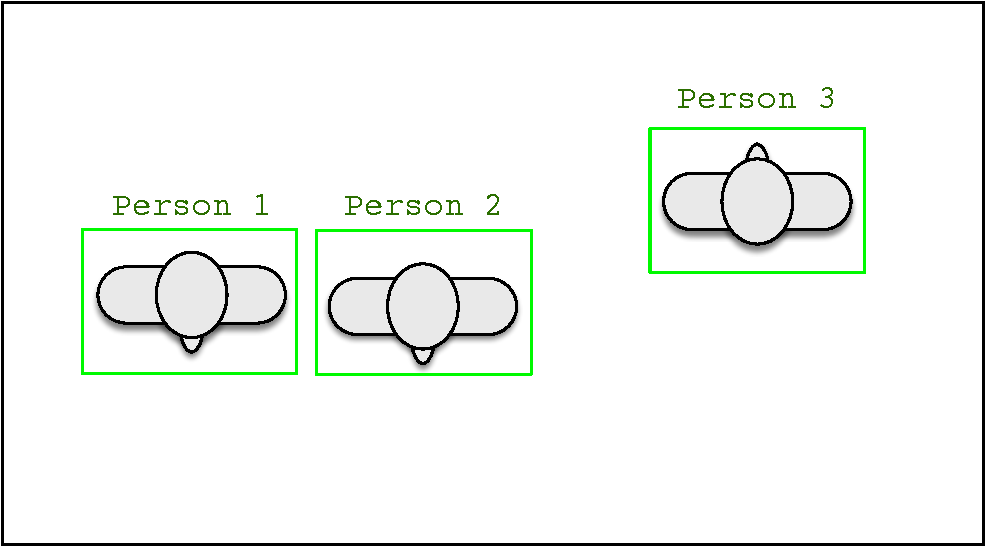
\includegraphics[width=\textwidth]{images/conturesConcept}
    \caption{Obraz snímanej scény}
  \end{minipage}
\end{figure}

% \section{Výber snezora (kamery)}
% Výber vhodného snímača priestoru virtuálnej brány je veľmi dôležitý. Ak senzor bude snímať dáta, ktoré sú enormne zaťažené šumom, realizácia funkčného algoritmu bude veľmi náročná, v niektorý prípadoch až nemožná. Táto práca sa zameriava na dva typy vhodných kamier \textbf{3D kamery} a\textbf{ 2D  RGB kamery}.

\section{Výber hĺbkového snímača}
Keďže  koncept snímania priestoru sa opiera o snímanie z výšky, veľmi silným kandidátom sú aktívne 3D kamery. Veľká výhoda je meranie na základe tvorby hĺbkového obrazu(kapitola XXX). Vďaka tomu, má meranie vysokú presnosť, nepotrebuje osvetlenie priestoru ani kontrastné prostredie.  Ďalšou veľkou výhodov je informácia o výške osoby, ktorá prechádza. Táto informácie je použiteľná v mnohých aspektoch ďalšieho spracovania. Na druhej strane technológia aktívneho 3D hĺbkomera je náchylná na priame slnečné lúče. Tie dokážu merania veľmi znehodnotiť. Vo svojej práci som otestoval tri rôzne aktívne hĺbkomery: 

\begin{itemize}
\item Kinect 360
\item Orbbec Astra S
\item Intel RealSence SR300

\end{itemize}


\subsection{Základné informácie o testovaných hĺbkomeroch}
\subsubsection{Kinect 360}
Kamera sníma frekvenciou 30 Hz. Hĺbka je snímaná s presnosťou na 11 bitov, čiže hĺbka jedného pixela môže nadobudnúť hodnoty od 0 do 2047.  Pracovný rozsah senzora je  1,2 - 3,5 metra.  Využíva technológiu vyvinutú firmou PrimaSence. V ľavej časti senzora sa nachádza IR projektor s vlnovou dĺžkou svetla 830nm. Generátor kóduje informáciu do svetelných vzorov, ktoré sa odrazom od predmetov pred senzorom deformujú. Odraz IR svetla je zachytený senzorom v pravej časti senzora a z veľkosti deformácii je vypočítaná hĺbková mapa. Používa USB 2.0 rozhranie. 

Kedže od spoločnosti Microsoft neexistuje oficialna podpora operačných systémov Unixového typu, na čítanie obrazu z kamery bola použitá knižnica \textit{libfreenect} ktorá je vyvíjaná a podporovaná komunitným spôsobom. Bola testovaná na RaspberryPI v3 s opereačným systémom Rasbian a MacOS Sierra. Použitá knižnica fungovala spoľahlivo. Na raspberry PI občasne vznikala menšia latencia spôsobená nižším výkonom.  

Výrazný problémom pri používaní tohoto hĺbkomeru je jeho veľkosť, váha, nutnosť externého napájania. Ďalší problém sa týka dostupnosti senzora. Senzor je zastaralí a už sa nevyrába. Cena sa momentálne stále drží na úrovni 150 eur. 

\subsubsection{Orbbec Astra S}
Ide o kameru, ktorá má veľmi podobný princíp funkčnosti ako kinect, čiže technológia je založená na vysielaní štrukturovaného svetla. Pracovný rozsah senzora je 0.4 – 2 metra. Kamera je pomerne malá a nepotrebuje externé napájanie. Používa USB 2.0 rozhranie. 

Knižnice od spoločnosť Orbbec má veľmi dobrú podporu všetkých operačných systémov. Cena 150 eur. 


\subsubsection{Intel RealSence SR300}
Je kamera, ktorá sa pomerne dosť líši od predchádzajúcich dvoch. Hlavným rozdielom je, že používa USB 3.0 čo znamená, že posiela väčšie množstvo dát a nieje možné ho pripojiť na RaspberyPi. Technológia snímania je založená na štrukturovanom svetle, podobne ako v predchádzajúcich dvoch prípadoch. Pracovný rozsah kamery je 25 až 70 cm. Cena kamery je tiež okolo 150 eur. 

\subsection{Porovnanie z hľadiska zorného poľa kamier}
Prvým parametrom porovnávania je \textbf{zorné pole kamier}. Každá hĺbková kamera, podobne ako klasické RGB kamery, majú zorný uhol daný použitou optikou kamery, hĺbkomery však majú navyše atribúty maximálnej a minimálnej vzdialenosti, na ktoré sú schopné vykonať meranie. Je to z dôvodu primárneho použiria kamery, pre ktoré ho výrobca vyrába. Napriklad \textit{Kinect 360} je určený pre hernú konzolu a detekciu celého tela, preto ma zorné pole veľmi veľké, aby mal hráč aj istú dávku voľnosti v pohybe. Presný opak kamery Kinect predstavuje \textit{Intel RealSence} ktorá je určená na aplikácie ovládania PC rôznymi gestami. Z dôvodu takéhoto obmedzenia nieje možné postaviť aplikáciu sledovania prechodov ľudí na jednom type kamery. (OBR 3.3) 



\begin{figure}[H]
\begin{center}
	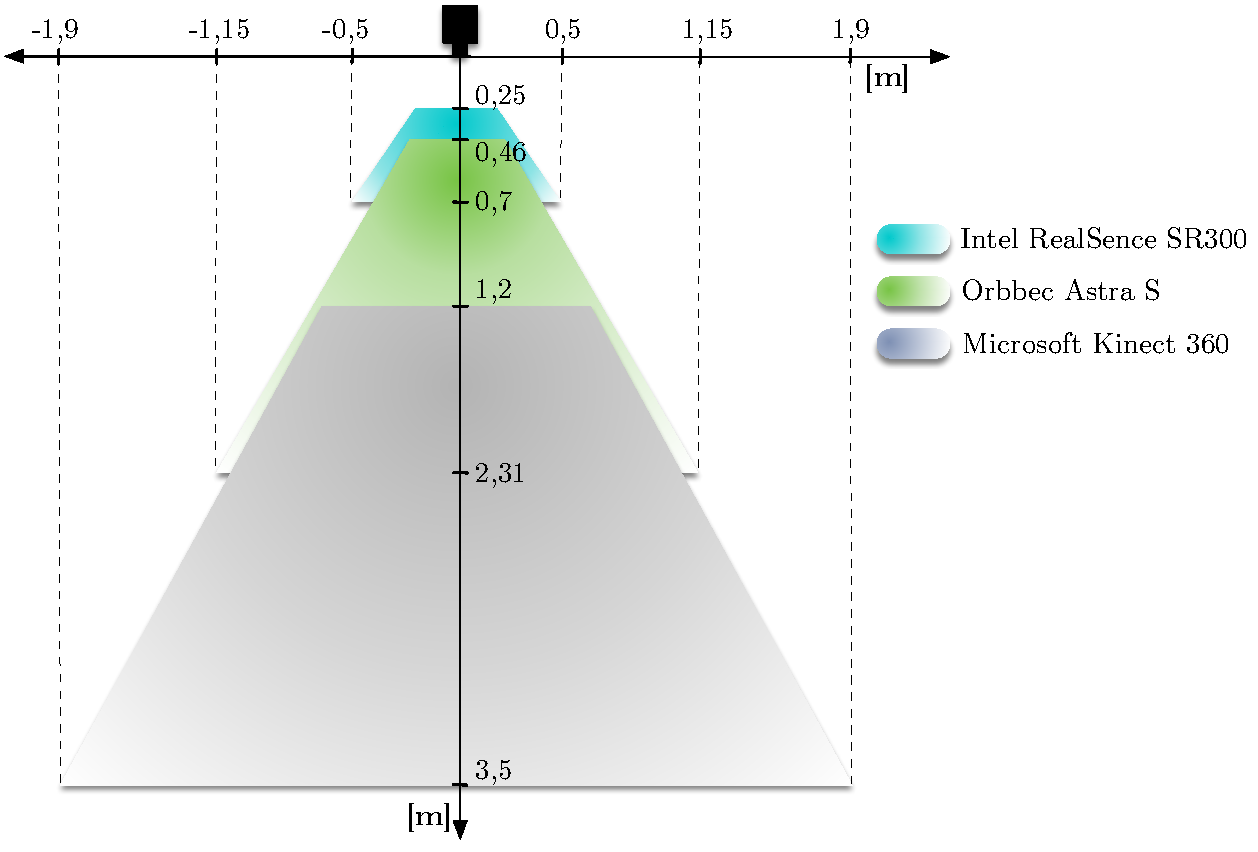
\includegraphics[scale=0.60]{images/camerasViews}
	\caption{Vizualizácia vertikálneho zorného pola hĺbkomerov}
	\end{center}
\end{figure}

Fyzické okolie virtuálnej brány nemusí dovoľovať umiestniť hĺbkomer do požadovanej snímacej výšky. Preto najlepším spôsobom je vyberať senzor špeciálne pre každé miesto nasadenia. Vďaka tomu je možné realizovať meranie od 2m do 4,5m.



\subsection{Testovanie kvality snímania}
Kvalita snímaného hĺbkového obrazu je veľmi dôležitým aspektom pre presnosť samotnej aplikácie. Keďže všetky testované hĺbkomery sú založené na technológii aktívnej triangulácie (kap x.x.x) v rôznych svetelných podmienkach môže kvalita vytvorených hĺbkových záznamov výrazne kolísať v závislosti na kamere. Z toho dôvodu boli vykonané testy, na základe ktorých je možné porovnanie jednotlivých snímačov. 

Predpokladajme, že každý bod scény, ktorý sa nachádza v zornom poli kamery sa premietne do šedotónového obrazu, v ktorom intenzita každého pixelu nadobúda hodnôt patriace do intervalu <0,254> v závislosti na vzdialenosti. Body, ktoré nebolo možné zmerať (nekonečne ďaleko, šum, materiál alebo tvar objektu atd...) nadobúdajú hodnotu 255 (biely pixel). Potom metódu, ktorá zráta priemerný počet pixlov s hodnotou 255 na snímku, je možné moužiť pre získanie \textbf{metriky} pre porovnanie. Avšak \textit{metóda pre výpočet hodnotiacej metriky konverguje k objektívnemu výsledku len vtedy, ak každý objekt scény sa nachádza v zornom poli kamery, ktoré udáva jej výrobca.}       

\subsubsection{Priebeh testovania}
Testovanie spočívalo v umiestnení kamier na náhodné miesto, kde sa v jednom okamihu nahrával ten istý bod na všetkých testovaných kamerách. Vďaka tomu je zaručené, že všetky kamery boli vystavené rovnakým podmienkam merania. Následne sa na vzniknuté záznamy aplikovala metóda pre výpočet metriky. Meranie sa konalo v piatich opakovaniach: 

\begin{enumerate}
\item test - pôda fakulty za denného svetla v zamračenom počasí
\item test - pôda fakulty za denného svetla s tlmeným slnečným žiarením
\item test - exteriér za denného svetla za slnečného počasia (v tieni)
\item test - exteriér za denného svetla za slnečného počasia s objektami v scéne
\item test - interiér za umelého osvetlenia
\end{enumerate}

\subsubsection{Výsledky testov}
Pri testovaní kamery \textit{Astra S} bola odhalená chyba. Kamera nieje schopná merať ľavý kraj o šírke 50 pixlov. Aby nedošlo k skresleniu v meraní, súčasťou hodnotiacej funkcie bolo odrezanie chybnej časti obrazu zo všetkých testovaných záznamov (aj na záznamoch z kamery Kinect). 

Ďalšia komplikácia nastala s kamerou \textit{Intel RealSence SR300}. Vzhľadom na jej extrémne malé zorné pole, nepodarilo sa splniť podmienku konvergencie hodnotiacej metódy. Ďalším problémom tejto kamery je nepripojiteľnosť na Raspberry PI z dôvodu absencie USB 3.0. Z uvedených dôvodov táto kamera nebola zaradená do výsledkov testov.  


\begin{figure}[H]
\begin{center}
	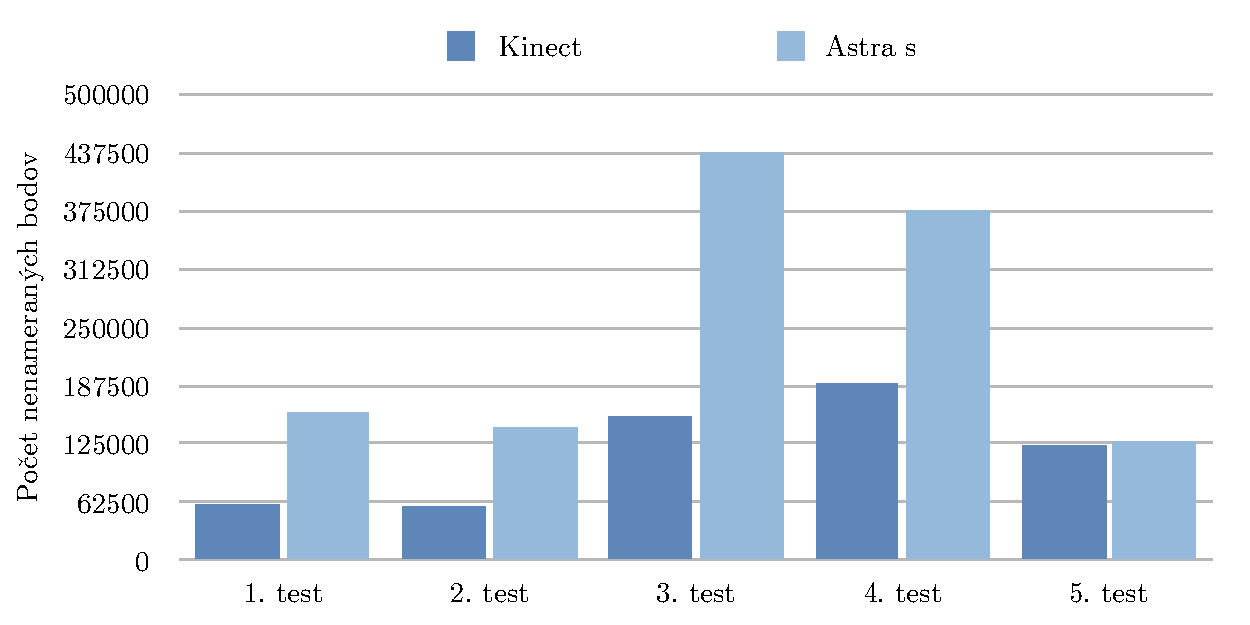
\includegraphics[scale=0.7]{images/noiseGraph}
	\caption{Vizualizácia vertikálneho zorného pola hĺbkomerov}
	\end{center}
\end{figure}

Z výsledkov vyplýva, že \textit{Kinect 360} je výrazne odolnejší v prípadoch interferencie denného svetla. Pri testoch za umelého alebo žiadneho osvetlenia je kvalita oboch kamier porovnateľná. 
















